% Options for packages loaded elsewhere
\PassOptionsToPackage{unicode}{hyperref}
\PassOptionsToPackage{hyphens}{url}
%
\documentclass[
]{book}
\usepackage{lmodern}
\usepackage{amsmath}
\usepackage{ifxetex,ifluatex}
\ifnum 0\ifxetex 1\fi\ifluatex 1\fi=0 % if pdftex
  \usepackage[T1]{fontenc}
  \usepackage[utf8]{inputenc}
  \usepackage{textcomp} % provide euro and other symbols
  \usepackage{amssymb}
\else % if luatex or xetex
  \usepackage{unicode-math}
  \defaultfontfeatures{Scale=MatchLowercase}
  \defaultfontfeatures[\rmfamily]{Ligatures=TeX,Scale=1}
\fi
% Use upquote if available, for straight quotes in verbatim environments
\IfFileExists{upquote.sty}{\usepackage{upquote}}{}
\IfFileExists{microtype.sty}{% use microtype if available
  \usepackage[]{microtype}
  \UseMicrotypeSet[protrusion]{basicmath} % disable protrusion for tt fonts
}{}
\makeatletter
\@ifundefined{KOMAClassName}{% if non-KOMA class
  \IfFileExists{parskip.sty}{%
    \usepackage{parskip}
  }{% else
    \setlength{\parindent}{0pt}
    \setlength{\parskip}{6pt plus 2pt minus 1pt}}
}{% if KOMA class
  \KOMAoptions{parskip=half}}
\makeatother
\usepackage{xcolor}
\IfFileExists{xurl.sty}{\usepackage{xurl}}{} % add URL line breaks if available
\IfFileExists{bookmark.sty}{\usepackage{bookmark}}{\usepackage{hyperref}}
\hypersetup{
  pdftitle={Lectures on Quantum Information Science},
  pdfauthor={Artur Ekert},
  hidelinks,
  pdfcreator={LaTeX via pandoc}}
\urlstyle{same} % disable monospaced font for URLs
\usepackage{longtable,booktabs}
\usepackage{calc} % for calculating minipage widths
% Correct order of tables after \paragraph or \subparagraph
\usepackage{etoolbox}
\makeatletter
\patchcmd\longtable{\par}{\if@noskipsec\mbox{}\fi\par}{}{}
\makeatother
% Allow footnotes in longtable head/foot
\IfFileExists{footnotehyper.sty}{\usepackage{footnotehyper}}{\usepackage{footnote}}
\makesavenoteenv{longtable}
\usepackage{graphicx}
\makeatletter
\def\maxwidth{\ifdim\Gin@nat@width>\linewidth\linewidth\else\Gin@nat@width\fi}
\def\maxheight{\ifdim\Gin@nat@height>\textheight\textheight\else\Gin@nat@height\fi}
\makeatother
% Scale images if necessary, so that they will not overflow the page
% margins by default, and it is still possible to overwrite the defaults
% using explicit options in \includegraphics[width, height, ...]{}
\setkeys{Gin}{width=\maxwidth,height=\maxheight,keepaspectratio}
% Set default figure placement to htbp
\makeatletter
\def\fps@figure{htbp}
\makeatother
\setlength{\emergencystretch}{3em} % prevent overfull lines
\providecommand{\tightlist}{%
  \setlength{\itemsep}{0pt}\setlength{\parskip}{0pt}}
\setcounter{secnumdepth}{5}
\usepackage{booktabs}
\ifluatex
  \usepackage{selnolig}  % disable illegal ligatures
\fi
\usepackage[]{natbib}
\bibliographystyle{apalike}

\title{Lectures on Quantum Information Science}
\author{Artur Ekert}
\date{2020-11-15}

\usepackage{amsthm}
\newtheorem{theorem}{Theorem}[chapter]
\newtheorem{lemma}{Lemma}[chapter]
\newtheorem{corollary}{Corollary}[chapter]
\newtheorem{proposition}{Proposition}[chapter]
\newtheorem{conjecture}{Conjecture}[chapter]
\theoremstyle{definition}
\newtheorem{definition}{Definition}[chapter]
\theoremstyle{definition}
\newtheorem{example}{Example}[chapter]
\theoremstyle{definition}
\newtheorem{exercise}{Exercise}[chapter]
\theoremstyle{remark}
\newtheorem*{remark}{Remark}
\newtheorem*{solution}{Solution}
\begin{document}
\maketitle

{
\setcounter{tocdepth}{1}
\tableofcontents
}
\hypertarget{overview}{%
\chapter*{Overview}\label{overview}}
\addcontentsline{toc}{chapter}{Overview}

\newcommand{\bra}[1]{\langle#1|}
\newcommand{\ket}[1]{|#1\rangle}

\hypertarget{quantum-interference}{%
\chapter{Quantum interference}\label{quantum-interference}}

\begin{quote}
About complex numbers, called probability amplitudes, that, unlike probabilities, can cancel each other out, leading to quantum interference and qualitatively new ways of processing information.
\end{quote}

The classical theory of computation does not usually refer to physics.
Pioneers such as Alan Turing, Alonzo Church, Emil Post and Kurt Gödel managed to capture the correct classical theory by intuition alone and, as a result, it is often falsely assumed that its foundations are self-evident and purely abstract.
They are not!\footnote{Computation is a physical process. Computation is a physical process. Computation is \ldots{}}

The concepts of information and computation can be properly formulated only in the context of a physical theory --- information is stored, transmitted and processed always by \emph{physical} means.
Computers are physical objects and computation is a physical process.
Indeed, any computation, classical or quantum, can be viewed in terms of physical experiments, which produce \textbf{outputs} that depend on initial preparations called \textbf{inputs}.
Once we abandon the classical view of computation as a purely logical notion independent of the laws of physics it becomes clear that whenever we improve our knowledge about physical reality, we may also gain new means of computation.
Thus, from this perspective, it is not very surprising that the discovery of quantum mechanics in particular has changed our understanding of the nature of computation.
In order to explain what makes quantum computers so different from their classical counterparts, we begin with the rudiments of quantum theory.

\hypertarget{two-basic-rules}{%
\section{Two basic rules}\label{two-basic-rules}}

Quantum theory, at least at some instrumental level, can be viewed as a modification of probability theory.
We replace positive numbers (probabilities) with complex numbers \(z\) (called \textbf{probability amplitudes}) such that the squares of their absolute values, \(|z|^2\), are interpreted as probabilities.

\begin{definition}
\protect\hypertarget{def:unlabeled-div-1}{}\label{def:unlabeled-div-1}

The correspondence between probability amplitude \(z\) and probability \(p=|z|^2\) is known as \textbf{Born's Rule}.

\end{definition}

The rules for combining amplitudes are very reminiscent of the rules for combining probabilities:

\begin{enumerate}
\def\labelenumi{\arabic{enumi}.}
\tightlist
\item
  Whenever something can happen in a sequence of independent steps, we multiply the amplitudes of each step.
\end{enumerate}

\begin{center}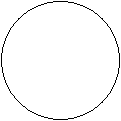
\includegraphics{quantum-site_files/figure-latex/unnamed-chunk-1-1} \end{center}

\begin{enumerate}
\def\labelenumi{\arabic{enumi}.}
\setcounter{enumi}{1}
\tightlist
\item
  Whenever something can happen in several alternative ways, we add the amplitudes for each separate way.
\end{enumerate}

That's it!
These two rules are basically all you need to manipulate amplitudes in any physical process, no matter how complicated.\footnote{We will, however, amend the two rules later on when we touch upon particle statistics.}
They are universal and apply to any physical system, from elementary particles through atoms and molecules to white dwarfs stars.
They also apply to information, since, as we have already emphasised, information is physical.
The two rules look deceptively simple but, as you will see in a moment, their consequences are anything but trivial.

\hypertarget{quantum-interference-the-failure-of-probability-theory}{%
\section{Quantum interference (the failure of probability theory)}\label{quantum-interference-the-failure-of-probability-theory}}

Modern mathematical probability theory is based on three axioms, proposed by Andrey Nikolaevich Kolmogorov (1903--1987) in his monograph with the impressive German title \emph{Grundbegriffe der Wahrscheinlichkeitsrechnung} (``Foundations of Probability Theory'').
The \textbf{Kolmogorov axioms} are simple and intuitive:\footnote{I always found it an interesting coincidence that the two basic ingredients of modern quantum theory, namely probability and complex numbers, were discovered by the same person, an extraordinary man of many talents: a gambling scholar by the name of Girolamo Cardano (1501--1576).}

\begin{enumerate}
\def\labelenumi{\arabic{enumi}.}
\tightlist
\item
  Once you identify all elementary outcomes, or events, you may then assign probabilities to them.
\item
  Probability is a number between \(0\) and \(1\), and an event which is certain has probability \(1\).
\item
  Last but not least, the probability of any event can be calculated using a deceptively simple rule --- the \emph{additivity axiom}:
\end{enumerate}

\begin{quote}
Whenever an event can occur in several mutually exclusive ways, the probability for the event is the sum of the probabilities for each way considered separately.
\end{quote}

Obvious, isn't it?
So obvious, in fact, that probability theory was accepted as a mathematical framework theory, a language that can be used to describe actual physical phenomena.
Physics should be able to identify elementary events and assign numerical probabilities to them.
Once this is done we may revert to mathematical formalism of probability theory.
The Kolmogorov axioms will take care of the mathematical consistency and will guide us whenever there is a need to calculate probabilities of more complex events.
This is a very sensible approach, apart from the fact that it does not always work!
Today, we know that probability theory, as ubiquitous as it is, fails to describe many common quantum phenomena.
In order to see the need for quantum theory let us consider a simple experiment in which probability theory fails to give the right predictions.

\hypertarget{the-double-slit-experiment}{%
\subsection{The double slit experiment}\label{the-double-slit-experiment}}

In a double slit experiment, a particle emitted from a source \(S\) can reach the detector \(D\) by taking two different paths, e.g.~through an upper or a lower slit in a barrier between the source and the detector.
After sufficiently many repetitions of this experiment we can evaluate the frequency of clicks in the detector \(D\) and show that it is inconsistent with the predictions based on probability theory.
Let us use the quantum approach to show how the discrepancy arises.

The particle emitted from a source \(S\) can reach detector \(D\) by taking two different paths, with amplitudes \(z_1\) and \(z_2\) respectively.
We may say that the upper slit is taken with probability \(p_1=|z_1|^2\) and the lower slit with probability \(p_2=|z_2|^2\).
These are two mutually exclusive events.
With the two slits open, probability theory declares (by the additivity axiom) that the particle should reach the detector with probability \(p_1+p_2= |z_1|^2+|z_2|^2\).
But this is not what happens experimentally!

Following the ``quantum rules'\,', first we add the amplitudes and then we square the absolute value of the sum to get the probability.
Thus, the particle will reach the detector with probability
\[
\begin{aligned}
  p = |z|^2 = |z_1 + z_2|^2
  & = |z_1|^2 + |z_2|^2
      + z_1^\star z_2 + z_1 z_2^\star
\\& = p_1 + p_2
      + |z_1||z_2|\left(
        e^{i(\varphi_2-\varphi_1)}
        + e^{-i(\varphi_2-\varphi_1)}
      \right)
\\& = p_1 + p_2
      + 2 \sqrt{p_1 p_2} \cos(\varphi_2-\varphi_1)
\\& = p_1 + p_2 + \mbox{interference terms}
\end{aligned}
\]
where we have expressed the amplitudes in their polar forms
\[
\begin{aligned}
  z_1 &= |z_1|e^{i\varphi_1}
\\z_2 &= |z_2|e^{i\varphi_2}.
\end{aligned}
\]
The appearance of the interference terms marks the departure from the classical theory of probability.
The probability of any two seemingly mutually exclusive events is the sum of the probabilities of the individual events, \(p_1 + p_2\), \emph{modified} by the \textbf{interference term} \(2 \sqrt{p_1p_2}\cos(\varphi_2-\varphi_1)\).
Depending on the \textbf{relative phase} \(\varphi_2-\varphi_1\), the interference term can be either negative (which we call \textbf{destructive} interference) or positive (\textbf{constructive} interference), leading to either suppression or enhancement of the total probability \(p\).

The algebra is simple; our focus is on the physical interpretation.
Firstly, note that the important quantity here is the \emph{relative} phase \(\varphi_2-\varphi_1\) rather than the individual values \(\varphi_1\) and \(\varphi_2\).
This observation is not trivial at all.
If a particle reacts only to the difference of the two phases, each pertaining to a separate path, then it must have, somehow, experienced the two paths, right?
Thus we cannot say that the particle has travelled either through the upper or the lower slit, because it has travelled through \emph{both}.
In the same way, quantum computers follow, in some tangible way, all computational paths simultaneously, producing answers that depend on all these alternative calculations.
Weird, but this is how it is!
Secondly, what has happened to the additivity axiom in probability theory --- what is wrong with it?
One thing that is wrong is the assumption that the processes of taking the upper or the lower slit are mutually exclusive.
In reality, as we have just mentioned, the two transitions \emph{both occur}, simultaneously.
However, we cannot learn this from probability theory, or any other a priori mathematical construct.
There is no fundamental reason why Nature should conform to the additivity axiom.
\footnote{According to the philosopher Karl Popper (1902--1994) a theory is genuinely scientific only if it is possible, in principle, to establish that it is false. Genuinely scientific theories are never finally confirmed because no matter how many confirming observations have been made observations that are inconsistent with the empirical predictions of the theory are always possible.}
We find out how nature works by making intelligent guesses, running experiments, checking what happens and formulating physical theories.
If our guess disagrees with experiments then it is wrong, so we try another intelligent guess, and another, etc.
Right now, quantum theory is the best guess we have: it offers good explanations and predictions that have not been falsified by any of the existing experiments.
This said, be assured that one day quantum theory will be falsified and we will have to start guessing again.

\hypertarget{superpositions}{%
\section{Superpositions}\label{superpositions}}

Amplitudes are more than just tools for calculating probabilities: they tell us something about physical reality.
When we deal with probabilities, we may think about them as numbers that quantify our lack of knowledge.
Indeed, when we say that a particle goes through the upper or the lower slit with some respective probabilities it does go through one of the two slits, we just do not know which one.
In contrast, according to quantum theory, a particle that goes through the upper and the lower slit with certain amplitudes does explore both of the two paths, not just one of them.
This is a statement about a real physical situation, about something that is out there and something we can experiment with.
The assumption that the particle goes through one of the two slits, but we do not know which one, is inconsistent with the experimental observations.
We have to accept that apart from some easy to visualise states, also known as the basis states, such as the particle at the upper slit or the particle at the lower slit, there are infinitely many other states, all of them equally real, in which the particle is in a \emph{superposition} of the two basis states.
This rather bizarre picture of reality is the best we have at the moment, and it works, at least for now. Physicists write such states as
\footnote{Dirac notation will likely be familiar to physicists, but may look odd to mathematicians or computer scientists. Love it or hate it (and I suggest the former), the notation is so common that you simply have no choice but to learn it, especially if you want to study anything related to quantum theory.}
\[
|\psi\rangle=\alpha |\text{at the upper slit}\rangle +\beta |\text{at the lower slit}\rangle,
\]
meaning the particle at the upper slit with amplitude \(\alpha\) and at the lower slit with amplitude \(\beta\). Mathematically, you can think about this expression as a vector \(|\psi\rangle\) in a two-dimensional complex vector space written in terms of the two basis vectors \(|\text{at the upper slit}\rangle\) and \(|\text{at the lower slit}\rangle\). You can also write this vector as a column vector with two complex entries \(\alpha\) and \(\beta\), but then you have to explain the physical meaning of the basis states. Here, we use the \(|\cdot\rangle\) notation, introduced by Paul Dirac in the early days of the quantum theory as a useful way to write and manipulate vectors. In Dirac notation you can put into the box \(|\phantom{0}\rangle\) anything that serves to specify what the vector is. It could be \(|\uparrow\rangle\) for spin up and \(|\downarrow\rangle\) for spin down, or \(|0\rangle\) for a quantum bit holding logical \(0\) and \(|1\rangle\) for a quantum bit holding logical \(1\), etc. As we shall see soon, there is much more to this notation.

\hypertarget{interferometers}{%
\section{Interferometers}\label{interferometers}}

\hypertarget{qubits-gates-and-circuits}{%
\section{Qubits, gates, and circuits}\label{qubits-gates-and-circuits}}

\hypertarget{quantum-decoherence}{%
\section{Quantum decoherence}\label{quantum-decoherence}}

\hypertarget{computation-deterministic-probabilistic-and-quantum}{%
\section{Computation: deterministic, probabilistic, and quantum}\label{computation-deterministic-probabilistic-and-quantum}}

\hypertarget{computational-complexity}{%
\section{Computational complexity}\label{computational-complexity}}

Is there a compelling reason why we should care about quantum computation?
It may sound like an extravagant way to compute something that can be computed anyway.
Indeed, your standard laptop, given enough time and memory, can simulate pretty much any physical process.
In principle, it can also simulate any quantum interference and compute everything that quantum computers can compute.
The snag is, this simulation, in general, is very inefficient.
And efficiency does matter, especially if you have to wait more than the age of the Universe for your laptop to stop and deliver an answer!
\footnote{The age of the Universe is currently estimated at 13.772 billion years.}

In order to solve a particular problem, computers (classical or quantum) follow a precise set of instructions --- an \textbf{algorithm}.
Computer scientists quantify the efficiency of an algorithm according to how rapidly its running time, or the use of memory, increases when it is given ever larger inputs to work on.
An algorithm is said to be \emph{efficient} if the number of elementary operations taken to execute it increases no faster than a polynomial function of the size of the input.
\footnote{Note that the technological progress alone, such as increasing the speed of classical computers, will never turn an inefficient algorithm (exponential scaling) into an efficient one (polynomial scaling). Why?}
We take the input size to be the total number of binary digits (bits) needed to specify the input.
For example, using the algorithm taught in elementary school, one can multiply two \(n\) digit numbers in a time that grows like the number of digits squared, \(n^2\).
In contrast, the fastest-known method for the reverse operation --- factoring an \(n\)-digit integer into prime numbers --- takes a time that grows exponentially, roughly as \(2^n\).
That is considered inefficient.

The class of problems that can be solved by a deterministic computer in polynomial time is represented by the capital letter \textsf{P}, for \emph{polynomial} time.
The class of problems that can be solved in polynomial time by a probabilistic computer is called \textsf{BPP}, for \emph{bounded-error probabilistic polynomial} time.
It is clear that \textsf{BPP} contains \textsf{P}, since a deterministic computation is a special case of a probabilistic computation in which we never consult the source of randomness.
When we run a probabilistic (a.k.a. randomised) computation many times on the same input, we will not get the same answer every time, but the computation is useful if the probability of getting the right answer is high enough.
Finally, the complexity class \textsf{BQP}, for \emph{bounded-error quantum polynomial}, is the class of problems that can be solved in polynomial time by a quantum computer.
Since a quantum computer can easily generate random bits and simulate a probabilistic classical computer, \textsf{BQP} certainly contains the class \textsf{BPP}.
Here we are interested in problems that are in \textsf{BQP} but not known to be in \textsf{BPP}.
The most popular example of such a problem is factoring.
A quantum algorithm, discovered by Peter Shor in 1994, can factor \(n\)-digit numbers in a number of steps that grows only as \(n^2\).
\footnote{It must be stressed that not all quantum algorithms are so efficient, in fact many are no faster than their classical counterparts. Which particular problems will lend themselves to quantum speed-ups is an open question.}
Since the intractability of factorisation underpins the security of many methods of encryption, Shor's algorithm was soon hailed as the first `killer application' for quantum computation: something very useful that only a quantum computer could do.
Since then, the hunt has been on for interesting things for quantum computers to do, and at the same time, for the scientific and technological advances that could allow us to build quantum computers.

\hypertarget{outlook}{%
\section{Outlook}\label{outlook}}

When the physics of computation was first investigated, starting in the 1960s, one of the main motivations was a fear that quantum-mechanical effects might place fundamental bounds on the accuracy with which physical objects could render the properties of the abstract entities, such as logical variables and operations, that appear in the theory of computation.
It turned out, however, that quantum mechanics itself imposes no significant limits, but does break through some of those that classical physics imposed.
The quantum world has a richness and intricacy that allows new practical technologies, and new kinds of knowledge.
In this course we will merely scratch the surface of the rapidly developing field of quantum computation.
We will concentrate mostly on the fundamental issues and skip many experimental details.
However, it should be mentioned that quantum computing is a serious possibility for future generations of computing devices.
At present it is not clear how and when fully-fledged quantum computers will eventually be built;
but this notwithstanding, the quantum theory of computation already plays a much more fundamental role in the scheme of things than its classical predecessor did.
I believe that anyone who seeks a fundamental understanding of either physics, computation or logic must incorporate its new insights into their world view.

\hypertarget{notes-and-exercises}{%
\section{Notes and Exercises}\label{notes-and-exercises}}

\hypertarget{supplement-physics-against-logic-via-beamsplitters}{%
\section{Supplement: Physics against logic, via beamsplitters}\label{supplement-physics-against-logic-via-beamsplitters}}

\hypertarget{supplement-quantum-interference-revisited-still-about-beamsplitters}{%
\section{Supplement: Quantum interference revisited (still about beamsplitters)}\label{supplement-quantum-interference-revisited-still-about-beamsplitters}}

\hypertarget{qubits}{%
\chapter{Qubits}\label{qubits}}

\hypertarget{measurements}{%
\chapter{Measurements}\label{measurements}}

\hypertarget{quantum-entanglement}{%
\chapter{Quantum entanglement}\label{quantum-entanglement}}

\hypertarget{quantum-algorithms}{%
\chapter{Quantum algorithms}\label{quantum-algorithms}}

\hypertarget{bells-theorem}{%
\chapter{Bell's theorem}\label{bells-theorem}}

\hypertarget{decoherence-and-elements-of-quantum-error-correction}{%
\chapter{Decoherence, and elements of quantum error correction}\label{decoherence-and-elements-of-quantum-error-correction}}

\hypertarget{density-matrices}{%
\chapter{Density matrices}\label{density-matrices}}

\hypertarget{quantum-channels-or-cp-maps}{%
\chapter{Quantum channels (or CP maps)}\label{quantum-channels-or-cp-maps}}

\hypertarget{quantum-error-correction-and-fault-tolerance}{%
\chapter{Quantum error correction and fault tolerance}\label{quantum-error-correction-and-fault-tolerance}}

  \bibliography{book.bib}

\end{document}
